\section{Set a table and clean it up [DSPL \& OPL]}
The robot has to set the table for a meal, and clean it up afterwards.

\subsection{Focus}
This test focuses on HRI, semantic mapping, object perception and manipulation.

\subsection{Setup}
\begin{itemize}
	\item \textbf{Location:} This test takes place inside the apartment, in a room with a table of the kind people sit to have a meal (e.g. kitchen's table).
	\item \textbf{Cutlery:} Cutlery and other appliances like carpets and napkins are stored inside a closed cupboard or similar type of furniture (e.g. inside a drawer).
	\item \textbf{Food:} Food and cleaning utensils are placed close to the table (e.g. in a rack or locker).
	\item \textbf{Cupboard:} The cupboard used to store the cutlery is located close to the table.
	\item \textbf{Table:} The table may have some objects on top of it, like a carpet or a plate.
\end{itemize}

\subsection{Task}
\label{sattu:task}
%\begin{figure}[tbp]
\begin{figure}[h!]
	\centering
	\subfloat[Typical arena]{\label{fig:sattu_table1}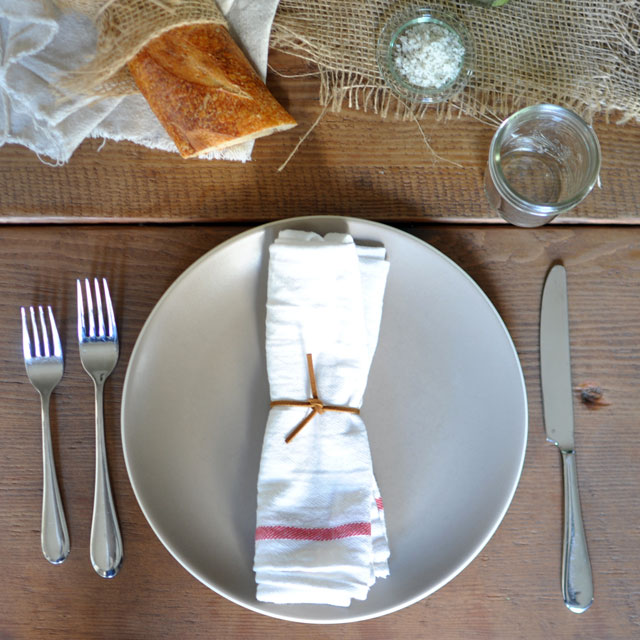
\includegraphics[height=46mm]{images/tablesetting1.jpg}} ~ 
	\subfloat[Typical objects]{\label{fig:sattu_table2}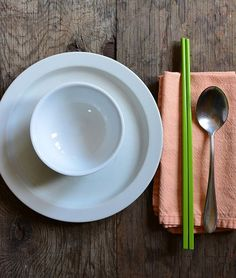
\includegraphics[height=46mm]{images/tablesetting2.jpg}}
	\caption{Table settings: (a) occidental, and (b) Japanese.}
	\label{fig:arena}
\end{figure}

\begin{itemize}
	\item[Part I:] Setting up the table
	\begin{enumerate}
		\item \textbf{Fetching command:} The operator requests the robot to set up the table. Optionally, the robot may ask the operator \textit{what has to be served}. The operator replies with the randomly selected (and undisclosed) option.

		\item \textbf{Setting the table:} The robot must safely and neatly place (i.e. without colliding with any existing object) all missing objects required for the meal. For example, carpet, fork, knife, spoon, and dish.

		% A remark is required here. If the robot will serve cereals, only carpet, bowl, and spoon would be necessary; while toast require dish, fork, and knife. How the table is set must depend on the requested meal (this will also save time).
		\item \textbf{Serving the meal:} If the robot asked the operator what to serve, it must proceed to place the order requested by the operator (e.g. pour cereal and milk in the bowl, or placing some slices of bread in the dish).

		% Yet another waste of time. First let's make sure robots can serve a proper breakfast, then we poke them.
		\item \textbf{Correcting object positions:} The operator will change the position of two objects on the table at any time before the placement of the last one. The robot must realize this change and rearrange the table to look neat.
	\end{enumerate}

	\item[Part II:] Cleaning up the table
	\begin{enumerate}
		\item \textbf{Fetching command:} After the meal, the operator requests the robot to clean up the table.

		% Actually this does not make any sense! Dirty dishes should be taken to the sink or dishwasher! The robot can be requested to distinguish between dirty and clean in a couple of years, maybe.
		\item \textbf{Clean the table:} After being instructed, the robot returns the objects to their original location, \textit{i.e.,} where they were found in the first place.
		% \item \textbf{Clean the table:} The robot must take all the dishes to the sink or dishwasher, as it was instructed.

		\item \textbf{Scrub spots and spills:} The robot must detect spots and spills on the table and clean them up using a cleaning cloth.
	\end{enumerate}
\end{itemize}

\subsection{Additional rules and remarks}
\label{sattu:add}
\begin{enumerate}
	\item \textbf{Startup:} The robot starts with a single voice command or via a start button (Section \refsec{rule:start_signal}). If the robot is unable to start it must be removed immediately.

	\item \textbf{Collisions:} Slightly touching the table is allowed, as well as slightly pushing some objects. However, driving over the objects or any other form of a major collision is not allowed, and the referees directly stop the robot (Section \refsec{rule:safetyfirst}).

	\item \textbf{Custom food:} Teams are allowed to provide their own food for preparing meal. However, it must be inspected by the TC at least 2 hours before the test.

	\item \textbf{Object list:} A total of 6 objects is considered, 3 of them considered easy to grasp (e.g., a cereal box, a cup, and a plate), while the remaining 3 hard to grasp (e.g., cutlery, napkins, and a basket with bread).

	\item \textbf{Opening the door:} If the robot is unable to open the door by itself, it may kindly ask the operator to do so.

	\item \textbf{Spots and Spills:} The referees will mess up the table right after it has been set, by spreading breadcrumbs, spilling some liquid, adding spots of jam, etc. It must be clear the robot has detected them and is trying actively to clean them, even though the cleaning may be unsuccessful.

	\item \textbf{Task variation:} The team may provide the referees a written set of at least 2 options for serving a meal (e.g. cereal and milk, sandwiches, toasts, Coffee and bread, etc.). These options must be written as possible answers to the robot question (step~\ref{sattu:s2} in section~\ref{sattu:task}). The correct execution of the specified variation should be clearly visible, e.g., choice of an object placed on the table.
\end{enumerate}

\subsection{Data recording}
  Please record the following data (See \refsec{rule:datarecording}):
  \begin{itemize}
   \item Images of recognized objects
   \item List of moved items
  \end{itemize}

\subsection{Referee instructions}

The referee needs to
\begin{itemize}
	\item Clean up any remaining object on the table.
	\item Place the objects the predefined locations.
	\item Close the closet door.
	\item Choose a random meal variation (when available).
	\item Ask the team whether they implemented a meal variation and choose randomly one of them.
\end{itemize}

\subsection{OC instructions}
During Setup days:
\begin{itemize}
	\item Provide official cutlery and appliances for training.
\end{itemize}

One day before the test:
\begin{itemize}
	\item Announce the food location.
	\item Announce the location for the cutlery and appliances.
\end{itemize}

2 hours before the test:
\begin{itemize}
	\item Collect from teams the set of meals their robot can serve.
	\item Place all objects and clear the table.
\end{itemize}

\newpage
\subsection{Score sheet}

The maximum time for this test is \textbf{10 minutes}. A maximum of 6 objects is
considered in this score sheet. 3 of those are easy to grasp, 3 are difficult to grasp (for a robot)

\begin{scorelist}

  \scoreheading{Meal variation}
  \scoreitem[1]{10}{For asking for the meal variation and confirming the choice}

	\scoreheading{Grasping objects}
	\scoreitem[12]{10}{For each successful grasp of any object (lifting it up to at least 5 cm for more than 10 seconds)}
	\scoreitem[12]{15}{For each successful grasp of an hard to grasp object (lifting it up to at least 5 cm for more than 10 seconds)}
        % Grasping = (* 12 (+ 10 15)) = 300

	\scoreheading{Placing objects}
	\scoreitem[6]{10}{For each successful placement of any object anywhere on the table (safely stands still for more than 10 seconds)}
	\scoreitem[6]{20}{For each successful placement of an hard to grasp object anywhere on the table (safely stands still for more than 10 seconds)}
        \scoreitem[1]{30}{For appropriately executing the operator's choice}
	\scoreitem[6]{-5}{For each collision of an object with another
        one on the table}
        % Placing = (+ (* 6 (+ 10 20)) 30) = 210

      \scoreheading{Cleaning up the  table}
	\scoreitem[6]{10}{For each successful placement of any object to its original location}
	\scoreitem[6]{20}{For each successful placement of an hard to grasp object to its original location(safely stands still for more than 10 seconds)}
        \scoreitem[1]{40}{For successfully cleaning up dirt and spill on the table}
        % Cleaning = (+ (* 6 (+ 10 20)) 40) = 220
	
% 	\scoreheading{Total task}
% 	\scoreitem[5]{40}{Place known object near known object of same class}
% 	\scoreitem[5]{50}{Place unknown object near unknown object of same class}

        \scoreheading{Bonus}
        \scoreitem[1]{15}{Open the door without human help}

	% (+ 10 Grasping Placing Cleaning Bonus))
	\setTotalScore{745}
\end{scorelist}

% \subsection{Score examples} 

% TODO

% \begin{itemize}
%  \item Robot A fails at all manipulation attemps but makes an excelent report, with the 5 known objects labeled correctly and the 5 pairs of unknown objects correctly, will get 
% $5*10 + 5*15 = 125$ points. 
%  \item Robot B that fails to recognize anything but does move all the objects from the table to anywhere in the cupboard receives $5*10 + 5*10 = 100$ points.
%  \item Robot C grasps a single unknown item (``Cookies''), places it at the correct position near the other ``Cookies'' and also makes the same excelent report as robot A will get 
% 10 points for grasping, 10 foor placing anywhere and an additional 5 for placing at the right location, so 25 for that single object.
% The  total for robot C is then 150 points.
% \end{itemize} 


% Local Variables:
% TeX-master: "Rulebook"
% End:


% Local Variables:
% TeX-master: "Rulebook"
% End:
